
\documentclass[aspectratio=169]{beamer}
\usetheme{Madrid}
\usecolortheme{default}
\usepackage{amsmath,amssymb,booktabs}
\usepackage[ruled,vlined]{algorithm2e}
\usepackage{graphicx}
\usepackage{ctex}
\usepackage{hyperref}
\hypersetup{
    colorlinks=true,        % 彩色链接
    linkcolor=blue,         % 内部链接颜色
    urlcolor=red,           % URL链接颜色
    citecolor=green,        % 引用颜色
    linkbordercolor={1 0 0} % 链接边框颜色（当colorlinks=false时）
}
\usepackage{microtype}
\usepackage{multirow}

% ---------------------------------------------------------------------------
% 排版与版式：统一间距与列表样式，避免拥挤
% ---------------------------------------------------------------------------
\setbeamertemplate{navigation symbols}{}
\setbeamertemplate{footline}[frame number]
\AtBeginSection[]{
  \begin{frame}{目录}
    \tableofcontents[currentsection]
  \end{frame}
}
\setlength{\leftmargini}{1.2em}
\setlength{\itemsep}{0.4em}
\setlength{\parskip}{0.35em}
\setbeamertemplate{itemize item}{\scriptsize\raise0.5pt\hbox{$\bullet$}}
\setbeamertemplate{enumerate item}{\insertenumlabel.}
\addtobeamertemplate{block body}{}{\vspace{0.3em}}

% 表格与公式周围留白
\setlength{\abovedisplayskip}{0.6em}
\setlength{\belowdisplayskip}{0.6em}
\setlength{\abovedisplayshortskip}{0.3em}
\setlength{\belowdisplayshortskip}{0.3em}

\usepackage{xcolor}
\newcommand{\redtwo}{\textcolor{red}{2}}
\newcommand{\highlight}[1]{\textcolor{blue!70!black}{\textbf{#1}}}
\graphicspath{{./}{figures/}}


\title{LLM 显存占用分析}
\subtitle{训练与推理过程中的内存需求与优化}
\author{\href{https://b23.tv/a0Bb9Z1}{Bilibili 以往的月}}
\institute{\href{https://maosong.website/}{Homepage}}
\date{\today}

\begin{document}

% ---------------------------------------------------------------------------
\frame{\titlepage}

% ---------------------------------------------------------------------------
% 目录：可补充「预计每节 2–3 分钟」等时间提示（讲稿用）
% ---------------------------------------------------------------------------
\begin{frame}{目录}
  \tableofcontents
\end{frame}

% ===========================================================================
\section{Motivation}
% ===========================================================================

% 补充：可口头说明「memory-bound 指访存成为瓶颈，compute-bound 指算力成为瓶颈」
\begin{frame}{Why Memory Matters}

  \begin{block}{A simple problem}
      假如我有一张80GB的显卡，我想训练/推理一个4B的模型，我应该设置多大的batch size 和sequence length?
  \end{block}

  在这个tutorial中，我们将基于这个问题来进行思考和分析。我们考虑更一般的问题形式：

  \begin{block}{Motivation}
    在训练和推理时 LLM 所需要的内存是多少？如何进行优化内存占用？
  \end{block}

  我们将先介绍训练/推理阶段的内存计算，再针对可优化部分进行分析并介绍相应优化算法。
\end{frame}

\section{Background}

\begin{frame}{Transformer Architecture}
    \begin{columns}
    \column{0.4\textwidth}
    \centering
        以Qwen3\cite{yang2025qwen3technicalreport}为例，现代LLM的架构如右图所示。其中具体的模块不同的模型可能有改动。

    \column{0.5\textwidth}
    \centering
    \begin{figure}
        \centering
        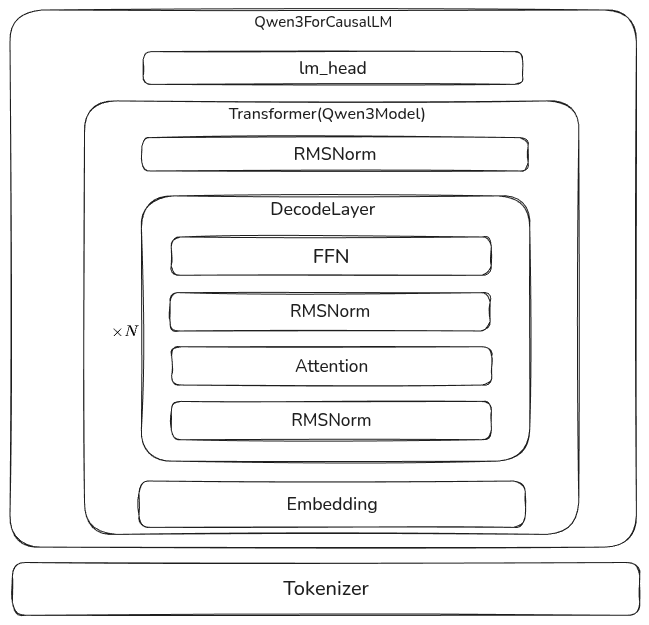
\includegraphics[width=0.9\linewidth]{LM_architecture.png}
        \caption{Architecture of Qwen3}
        \label{fig:placeholder}
    \end{figure}
    \end{columns}
    

   
\end{frame}

\begin{frame}{Notation}
  \small
  与参数量、FLOPs 计算所用记号一致；参数量 $P$ 的推导见 \href{https://maosong.website/p/llm-parameter-computation/}{LLM parameter analysis}。
  \vspace{0.6em}
  \begin{center}
    \begin{tabular}{@{}cl@{}}
      \toprule
      \textbf{变量} & \textbf{含义} \\
      \midrule
      $P$   & number of parameters \\
      $L$   & layers \\
      $V$   & vocabulary size \\
      $d$   & hidden size \\
      $d_{\mathrm{ff}}$ & FFN hidden size \\
      $s$   & sequence length \\
      $b$   & batch size \\
      $h$   & number of attention heads \\
      $d_h$ & attention head dimension \\
      \bottomrule
    \end{tabular}
  \end{center}
\end{frame}

\begin{frame}{Assumption}
  \begin{enumerate}
    \item 若无特别说明，使用 \textbf{BF16/FP16}，每个参数 $\redtwo$ byte。
    \item 不使用 dropout（与现代大模型设定一致）。
    \item Attention 基于原始multi-head attention.
    \item FFN基于SwiGLU.
  \end{enumerate}
  % 补充：可说明「BF16 兼顾范围与精度，FP16 易溢出，FP32 显存翻倍」
\end{frame}


\section{Training Memory Analysis}

\begin{frame}{Training Memory Componenets}
    训练部分的内存占用由四部分组成，如下所示
    \begin{align}
    \text{training\_memory} &= \text{weight} \\
    &+ \text{activation} \\
    &+ \text{optimizer} \\
    &+\text{gradient}
    \end{align}
    \textbf{Weights}：$\boxed{\redtwo P}$.

    \textbf{Gradients}（与权重同精度）：$\boxed{\redtwo P}$.
\end{frame}


\begin{frame}{Optimizer states}

    \begin{columns}
        \column{0.4\textwidth}
        \textbf{AdamW} 优化器：
      \begin{itemize}
        \item 一阶动量：$\redtwo P$，
        \item 二阶动量：$\redtwo P$,
        \item 合计：$2\times \redtwo P = \boxed{4P}$.
      \end{itemize}

      \column{0.5\textwidth}
      \begin{algorithm}[H]
        \KwIn{$\alpha$, $\lambda$, $\beta_1, \beta_2 \in [0,1)$, $\epsilon$, $\theta_0$}
        \KwOut{$\theta_t$}
        
        $m_0 \leftarrow 0$, $v_0 \leftarrow 0$, $t \leftarrow 0$\;
        
        \While{Not converge}{
            $t \leftarrow t + 1$\;
            $g_t \leftarrow \nabla_\theta f_t(\theta_{t-1})$\;
            $m_t \leftarrow \beta_1 \cdot m_{t-1} + (1 - \beta_1) \cdot g_t$\;
            $v_t \leftarrow \beta_2 \cdot v_{t-1} + (1 - \beta_2) \cdot g_t^2$\;
            $\hat{m}_t \leftarrow \frac{m_t}{1 - \beta_1^t}$\;
            $\hat{v}_t \leftarrow \frac{v_t}{1 - \beta_2^t}$\;
            $\theta_t \leftarrow \theta_{t-1} - \alpha \left( \frac{\hat{m}_t}{\sqrt{\hat{v}_t} + \epsilon} + \lambda \theta_{t-1} \right)$\;
        }
        \caption{AdamW\cite{loshchilov2019decoupledweightdecayregularization}}
      \end{algorithm}
  \end{columns}
\end{frame}

% 补充：可画简图「前向 → 存 a_l → 反向用 a_l 算 dW_l」
\begin{frame}{Activation}
  \begin{block}{Motivation}
      激活值是前向传播过程中计算得到的中间结果，用于在反向传播时计算梯度。
  \end{block}
  
  我们仅针对linear layer进行推导

  \begin{align*}
    \text{forward}&\quad &\mathbf{z}_\ell = W_\ell\mathbf{a}_{\ell-1}+b_\ell,\quad \mathbf{a}_{\ell} = \phi(\mathbf{z}_\ell) \\
    \text{backward}&\quad&\frac{\partial \mathcal{L}}{\partial W_\ell}
    = \frac{\partial \mathcal{L}}{\partial \mathbf{z}_\ell}\cdot
    \frac{\partial \mathbf{z}_\ell}{\partial W_\ell}
    = \frac{\partial \mathcal{L}}{\partial \mathbf{z}_\ell} \boxed{\mathbf{a}_{\ell-1}}
  \end{align*}

  可以看到，计算第 $\ell$ 层关于$W_{\ell}$ 的梯度时需要其输入 $\mathbf{a}_{\ell-1}$，因此训练时需保存每个模块对应的输入，也就是激活值 (activation).
\end{frame}


\begin{frame}{Activation-Attention}
    \begin{columns}[c]
    \column{0.5\textwidth}
      \small
      按计算图（无优化）可得需保存的激活：
      \vspace{0.3em}
      \begin{itemize}
        \item Q/K/V 投影：共享输入 $\to$ $\redtwo bsd$
        \item $Q^\top K$：$Q,K$ 均需保存 $\to$ $2\times \redtwo bsd=4bsd$
        \item softmax 输入：$\redtwo bhs^2$
        \item weighted sum 输入：$\redtwo bhs^2 + \redtwo bsd$
        \item output projection 输入：$\redtwo bsd$
      \end{itemize}
      \vspace{0.4em}
      \textbf{Attention 合计：} $\boxed{10sbd + 4bhs^2}$.

    \column{0.5\textwidth}
      \centering
      \vspace{-0.3em}
      % 若同目录下有 Attention-computation-graph.png，取消下行注释：
      \IfFileExists{Attention-computation-graph.png}{%
        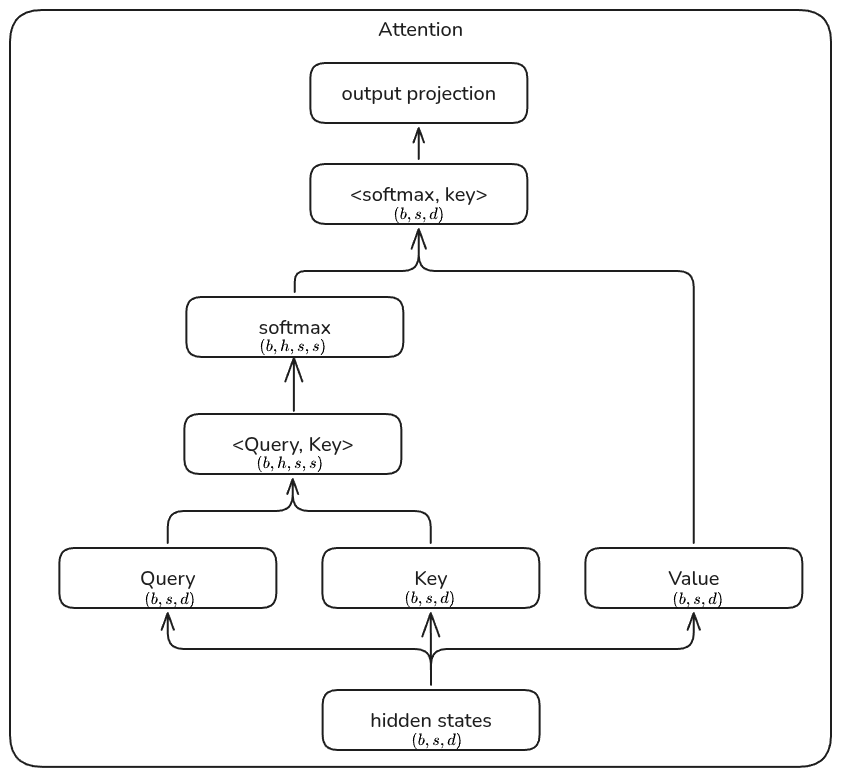
\includegraphics[width=\textwidth]{Attention-computation-graph.png}%
      }{%
        \fbox{\parbox[c][0.34\textheight][c]{0.92\textwidth}{\centering\footnotesize 图：Attention 计算图（缺少图片文件）}}%
      }
  \end{columns}
\end{frame}

\begin{frame}{Activation-FFN \& LayerNorm}
    \begin{columns}[c]
    \column{0.55\textwidth}
      \small
      \textbf{FFN}（SwiGLU，assume $d_{\mathrm{ff}}=4\,d$）：
      \begin{itemize}
        \item 第一层输入 $\redtwo\, sbd$
        \item SwiGLU 输入 $\redtwo \times d_{ff}\times d=8\,sbd$
        \item 第二层输入 $\redtwo \times d_{ff}\times d=8\,sbd$
        \item 合计：$\boxed{18sbd}$
      \end{itemize}
      \vspace{0.4em}
      \textbf{LayerNorm}：保存输入 $\to$ $\boxed{\redtwo bsd}$.
      
    \column{0.45\textwidth}
      \centering
      \vspace{-0.3em}
      % 若同目录下有 FFN-computation-graph.png，取消下行注释：
        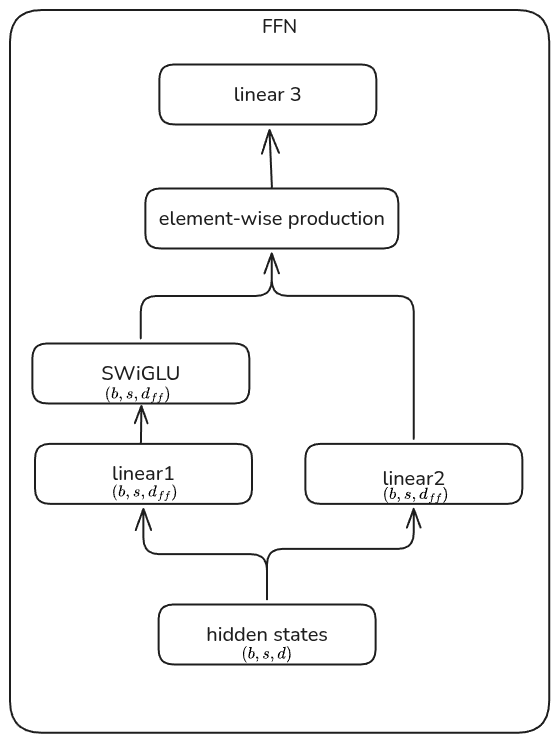
\includegraphics[width=0.8\textwidth]{FFN-computation-graph.png}%
  \end{columns}
\end{frame}

\begin{frame}{Activation-Output}
    \begin{columns}[c]
    \column{0.55\textwidth}
      \small
      \textbf{Output} 包含以下组成部分：
      \begin{itemize}
        \item \textbf{FinalNorm} 输入：$\redtwo bsd$
        \item \textbf{lm\_head} 输入：$\redtwo bsd$
        \item \textbf{Loss} 输入：$\redtwo bsV$
      \end{itemize}
      \vspace{0.4em}
      合计：$\boxed{4bsd+2bsV}$。
    \column{0.45\textwidth}
      \centering
      \vspace{0.3em}
      \includegraphics[width=0.8\textwidth]{Output-computation-graph.png}
  \end{columns}
\end{frame}

\begin{frame}{Activation-Total}
    \small
  我们将上面的结果汇总在一起，得到\footnote{Qwen3中，$2V/32dL= 6\%$, $32dL/4hsL=2.5\%$.}
  \begin{align}
    \mathrm{activation}
    &= L \cdot \mathrm{transformer\_block} + \mathrm{output}\\
    &= L \cdot(\mathrm{Pre\_Norm} + \textcolor{red}{Attention} + \mathrm{Post\_Norm} + \mathrm{FFN}) + \mathrm{output}\\
    &=\boxed{bs(32dL+\textcolor{red}{4hsL}+4d+2V)}\\
    &\approx bsL(32d+\textcolor{red}{4hs})\\
    &\approx \textcolor{red}{4bs^2hL}
  \end{align}
  我们可以看到，未优化的情况下，$\mathrm{activation}\propto bs^2$. 这里 $s^2$ 主要由 attention 部分产生，后续 flash attenion 就针对这一点进行了优化。
\end{frame}

\begin{frame}{Total Training Memory}
    我们将上面的结果进行汇总得到
    \begin{align}
    \text{training\_memory} &= \text{weight}
    + \text{activation}
    + \text{optimizer}
    +\text{gradient}\\
    &= 2P +  bs(32dL+4hsL+4d+2V) + 4P+2P\\
    &= 8P + bs(32dL+4hsL+4d+2V) \tag{exact}\\
    &\approx 8P+4bs^2hL
  \end{align}
  可以看到，训练阶段的内存占用分为固定部分 ($8P$) 和动态部分 ($4bs^2hL$), 动态部分主要是attention的缓存。
\end{frame}

\begin{frame}{Analysis}
    我们以Qwen3模型为例，得到如下热力图，batchh size越小，说明activation占用越高

    \begin{figure}
        \centering
        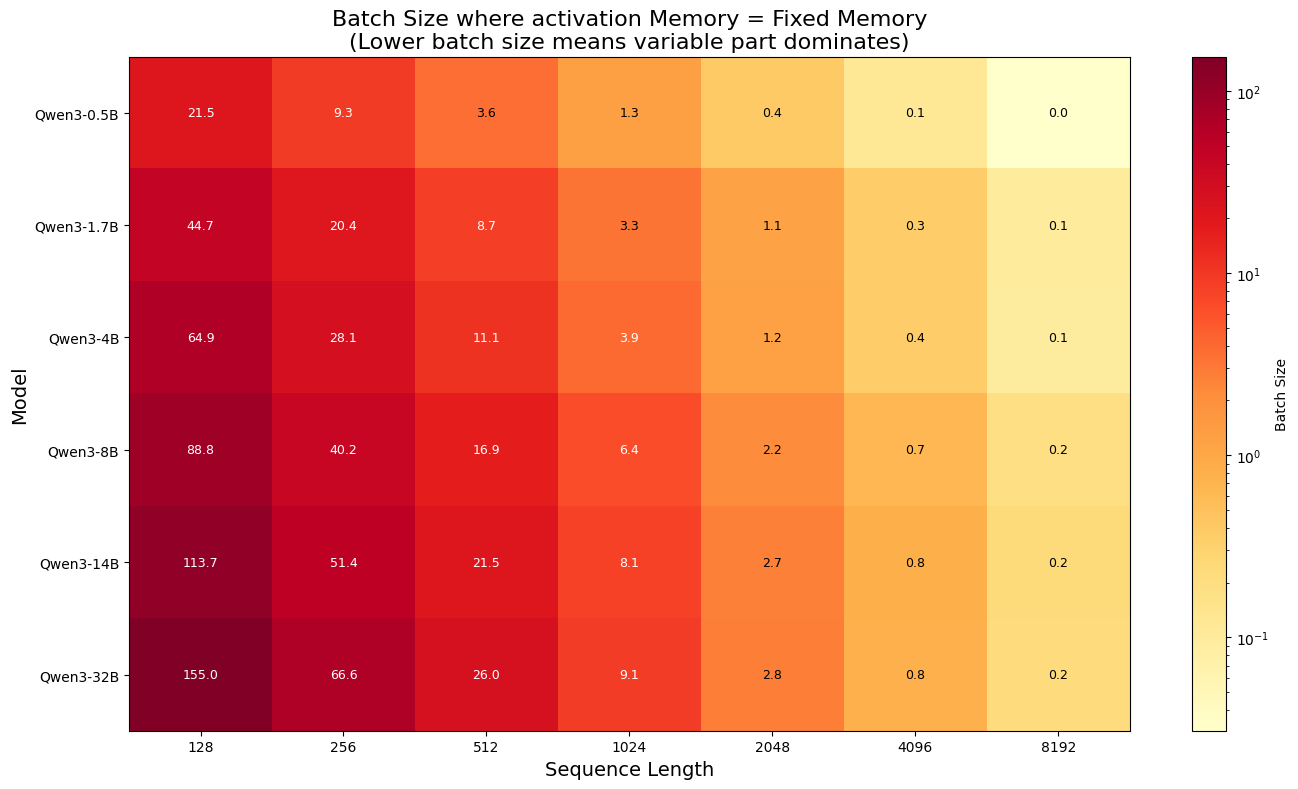
\includegraphics[width=0.5\linewidth]{qwen3_equal_points_heatmap.png}
        \caption{Comparison of activation memory with fixed memory}
        \label{fig:placeholder}
    \end{figure}
\end{frame}

\begin{frame}{Experiments}
    我们分别针对80GB的显卡计算Qwen3系列模型的最高配置：
    \begin{table}[]
        \begin{tabular}{cccccccc}
        \toprule
        Model      & $P$  & $L$ & $h$ & $s$ & predicted $b$  & actual $b$ \\
        \midrule
        Qwen3-0.6B & 0.6  & 28  & 16  & 512 & 68   & 34        \\
        \midrule
        Qwen3-1.7B & 1.7  & 28  & 16  & 512 & 42   & 28        \\
        \midrule
        Qwen3-4B   & 4    & 36  & 32  & 512 & 16   & 12        \\
        \midrule
        Qwen3-8B   & 8.1  & 36  & 32  & 512 & 4    & 2         \\
        \bottomrule
        \end{tabular}
    \end{table}
    其中 predicted $b$ 基于前面的准确公式计算得到；actual $b$ 通过实验验证得到。 （注意我们这里的prediction没有考虑任何优化手段与其他内存开销，因此与实际值有出入）
\end{frame}


\begin{frame}{Case Study}
    我们分别使用Qwen3-4B和Qwen3-8B来进行实验 ($b=1$, $s=512$), 结果如下\footnote{参考\href{https://zhuanlan.zhihu.com/p/677203832}{PyTorch显存可视化与Snapshot数据分析}}
    \begin{minipage}{0.48\textwidth}
        \begin{figure}
            \centering
            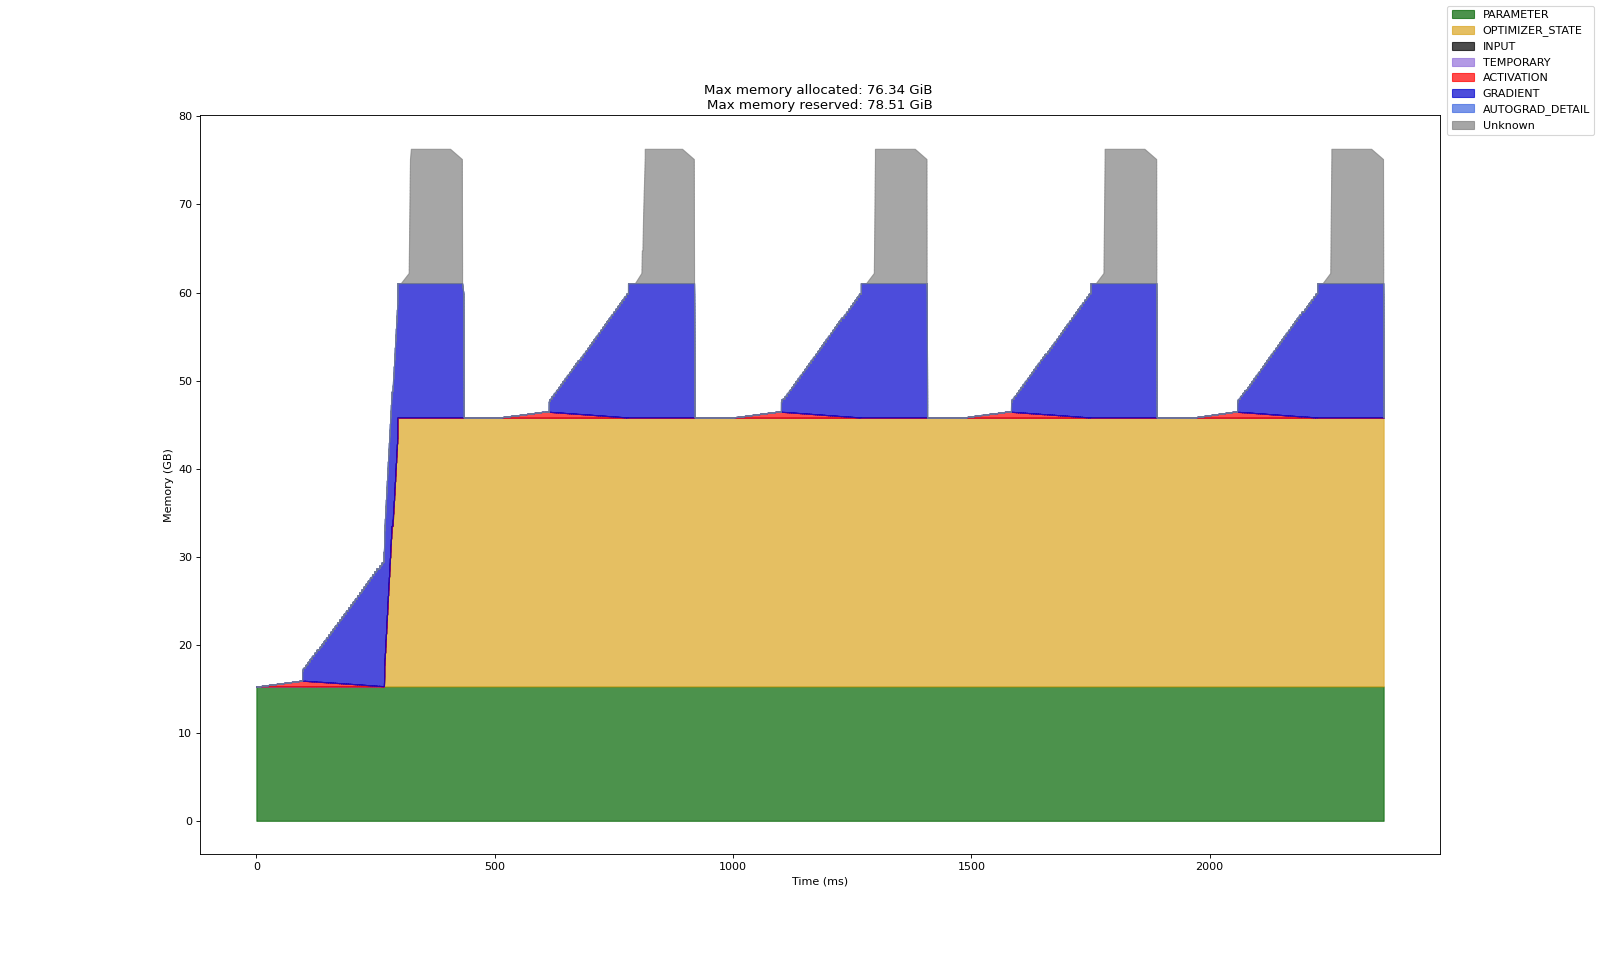
\includegraphics[width=\linewidth]{qwen3-8b-bs1-seq512.png}
            \caption{Memory profile of Qwen3-8B}
            \label{fig:placeholder}
        \end{figure}
    \end{minipage}
    \hfill
    \begin{minipage}{0.48\textwidth}
        \begin{figure}
            \centering
            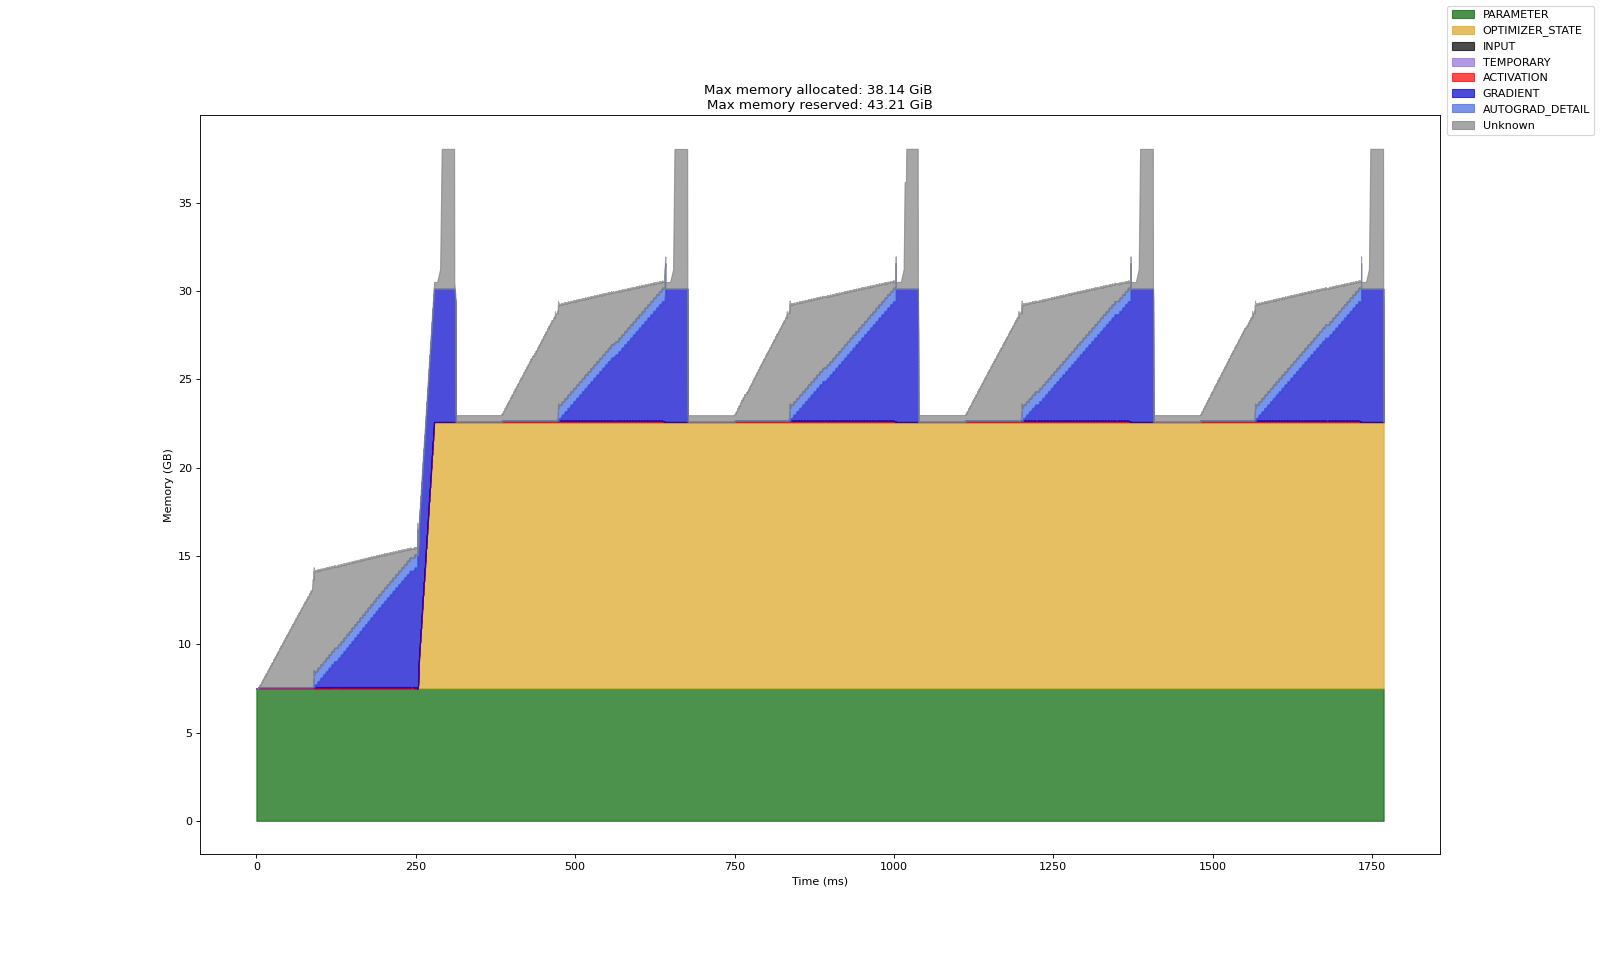
\includegraphics[width=\linewidth]{qwen3-4b-bs-1-seq-512.png}
            \caption{Memory profile of Qwen3-4B}
        \end{figure}
    \end{minipage}
\end{frame}



\section{Inference Memory Analysis}

\begin{frame}{Inference Components}
  Inference阶段内存占用主要与模型参数，KV cache两部分相关。
    \begin{align}
    \mathrm{Inference\_Memory}&= \mathrm{weight}\\
    &+ \mathrm{activation}\\
    &+ \mathrm{KV\ cache}
  \end{align}
  \begin{itemize}
    \item Weights：$\boxed{\redtwo P}$
    \item Activations（经验\footnote{见 \url{https://blog.eleuther.ai/transformer-math/}}，batch size=1）：$\approx 0.4P$
    \item KV cache：与序列长度相关，见后续分析。
  \end{itemize}
\end{frame}


\begin{frame}{KV Cache Mechanism}
  \small
  \begin{block}{Motivation}
      LLM 推理中为避免重复计算历史 token 的 key/value 而使用的\textbf{空间换时间}的缓存机制。
  \end{block}

  自回归时逐 token 生成，每步 attention 形式为（$\mathbf{q}_t$ 当前 query，$\mathbf{k}_{:,t}$/$\mathbf{v}_{:,t}$ 历史 K/V）：
  \begin{align*}
    \mathbf{q}_t &= W_Q\mathbf{x}_t,\quad
    \mathbf{k}_{:,t} = W_K[\mathbf{x}_1,\ldots,\mathbf{x}_t],\quad
    \mathbf{v}_{:,t} = W_V[\mathbf{x}_1,\ldots,\mathbf{x}_t]
  \end{align*}
  处理下一 token $\mathbf{x}_{t+1}$ 时只需在已有结果后追加当前步：
  \begin{equation*}
    \mathbf{k}_{:,t+1} = W_K[\mathbf{x}_1,\ldots,\mathbf{x}_{t+1}]=[\mathbf{k}_{:,t},\, W_K\mathbf{x}_{t+1}],\quad
    \mathbf{v}_{:,t+1} = W_V[\mathbf{x}_1,\ldots,\mathbf{x}_{t+1}]=[\mathbf{v}_{:,t},\, W_V\mathbf{x}_{t+1}]
  \end{equation*}
  缓存前，每生成一个 token 都重新计算 $\to$ 总计算量 $\sum_{t=1}^s \mathcal{O}(t) = \mathcal{O}(s^2)$；
  
  缓存后，每步只算当前token $W_K\mathbf{x}_{t+1}$、$W_V\mathbf{x}_{t+1}$ $\to$ 计算量 $\mathcal{O}(s)$、空间占用 $\mathcal{O}(s)$ —— \textbf{以空间换时间}。
  % 公式中两个 2：一层 K+V，以及每项 2 bytes (BF16)
\end{frame}

\begin{frame}{KV Cache Memory}
    对于 multi-head attention ，KV cache 的显存占用为：
  \begin{equation}
    \mathrm{Memory}(\mathrm{KV\ cache})
    = s \times 2 \times \redtwo \times L \times h \times d_h
    = \boxed{4sLhd_h}
  \end{equation}
  
  \textbf{因子含义：} $s$ 序列长， $2$ 为 K+V,  $L$ 层、$h$ 头、$d_h$ 头维度。

  \begin{block}{Remark}
      \begin{itemize}
    \item KV 占用与\textbf{模型配置}（$L,h,d_h$）和\textbf{序列长度} $s$ 都有关，token 越多占用越高。
    \item 实际中因 \textit{page granularity}、\textit{padding}、\textit{fragmentation} 往往略高于理论值。
    \item 长输出时 KV 占比会超过权重，成为推理瓶颈 $\to$ 见后续「KV Cache 优化」。
  \end{itemize}
  \end{block}
  

\end{frame}


\begin{frame}{Inference Memory}
综合前面分析，我们可以得到推理阶段的总内存为：
\begin{equation*}
    \boxed{
      \mathrm{Inference\_Memory}
      \approx 2.4P + 4sLhd_h
    }
  \end{equation*}
  可以看到，推理阶段也由固定部分（参数量，activation）以及动态部分（KV cache）组成。
\end{frame}


\begin{frame}{Experiments}
  \small
    我们仍然使用Qwen3系列来进行实验（未考虑任何优化，仅考虑KV cache和prefilling），结果如下：
    \begin{figure}
      \centering
      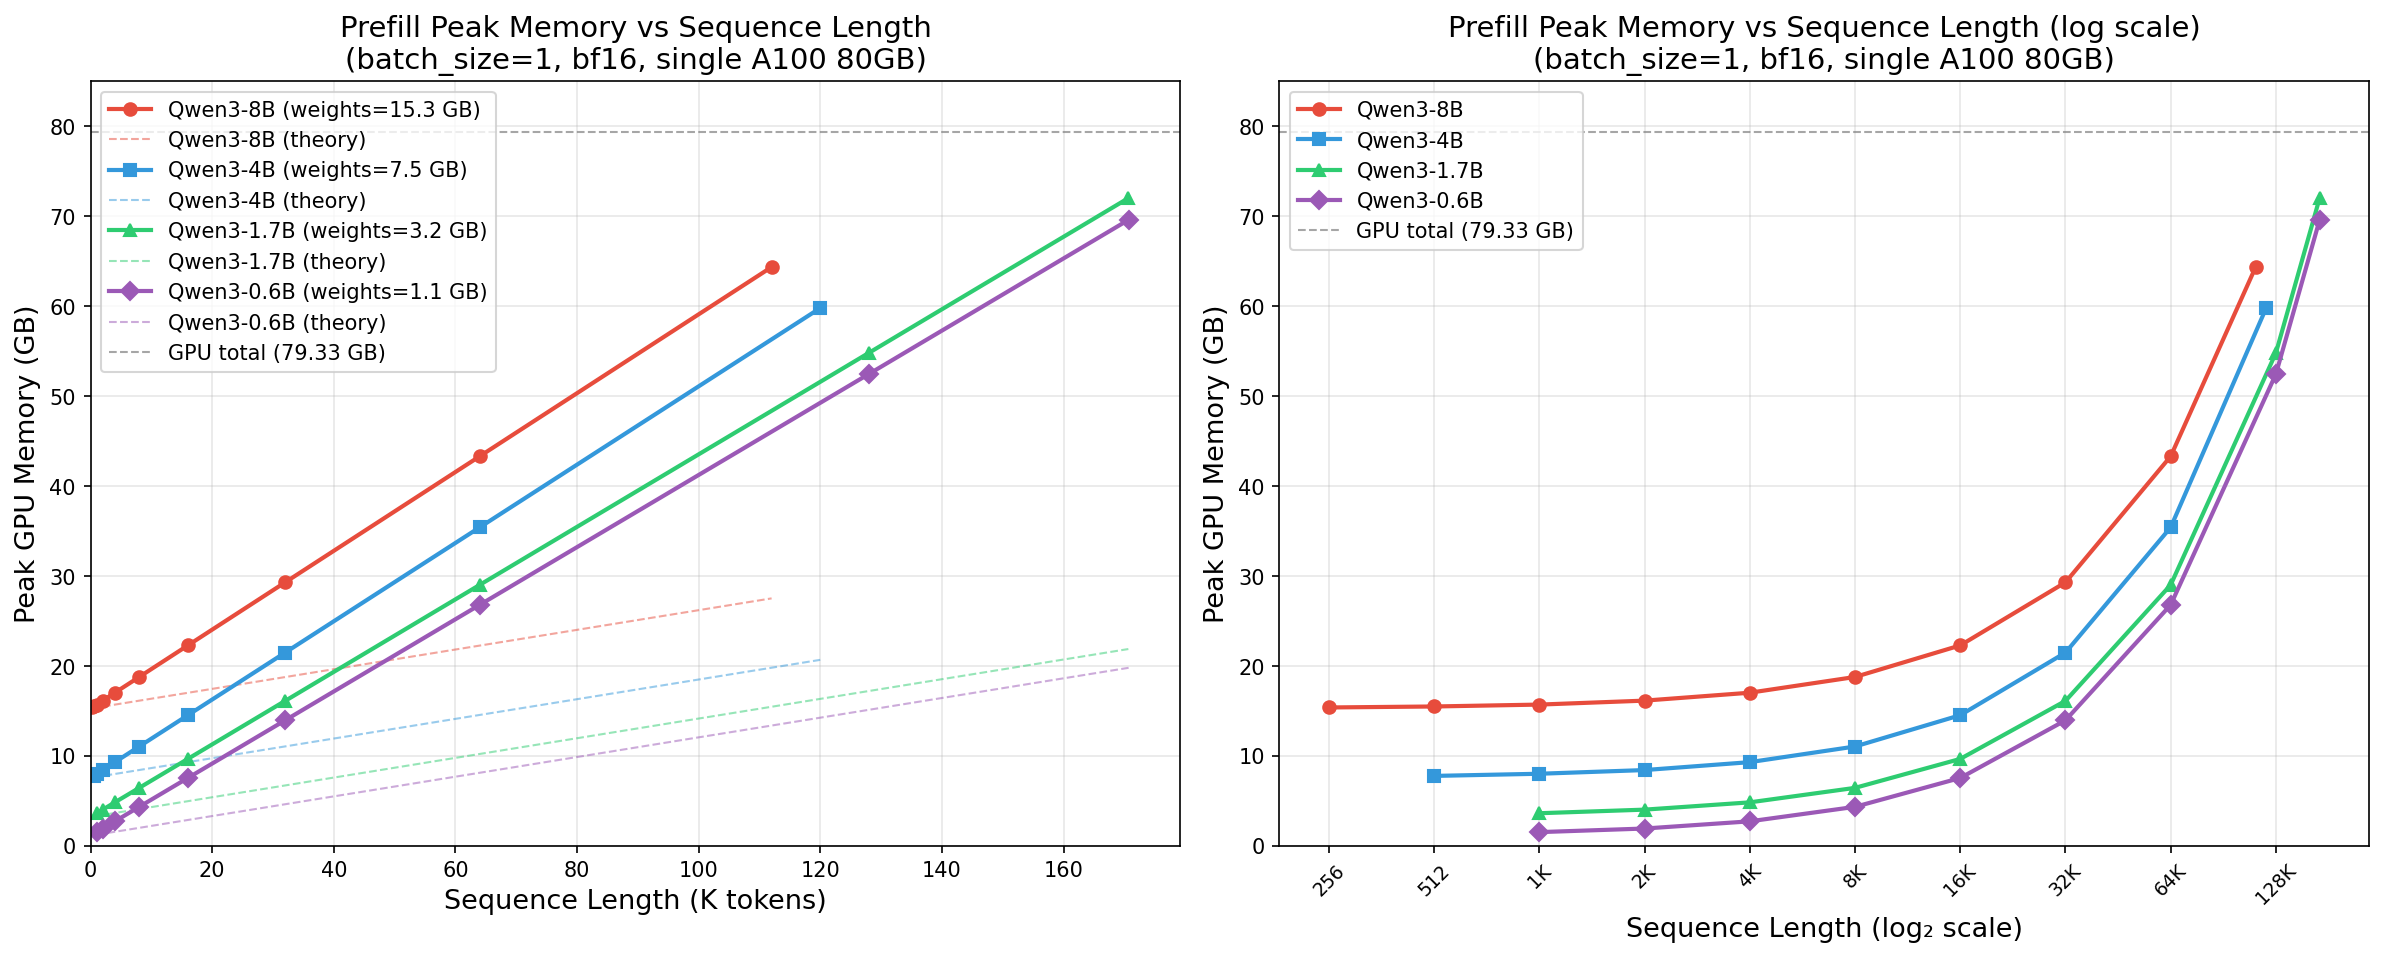
\includegraphics[width=0.8\linewidth]{seq_len_memory_curve.png}
      \caption{Memory profile for Qwen3 series}
    \end{figure}
    注意这里的peak memory实际上并不能和KV cache的显存占用完全对应，因为peak memory还包括了attention的临时显存等。
\end{frame}


\begin{frame}{Dynamic v.s. Static}
  \small
  接下来我们看一下模型权重与KV cache的显存占用情况。
  由于 Qwen3 的 KV cache计算为 $4sLh_{kv}d_h$, 而不同模型只有 $L$ 不一样，因此对于更大的模型，KV cache显存占用超过模型权重的上下文长度更高。
  \begin{figure}
    \centering
    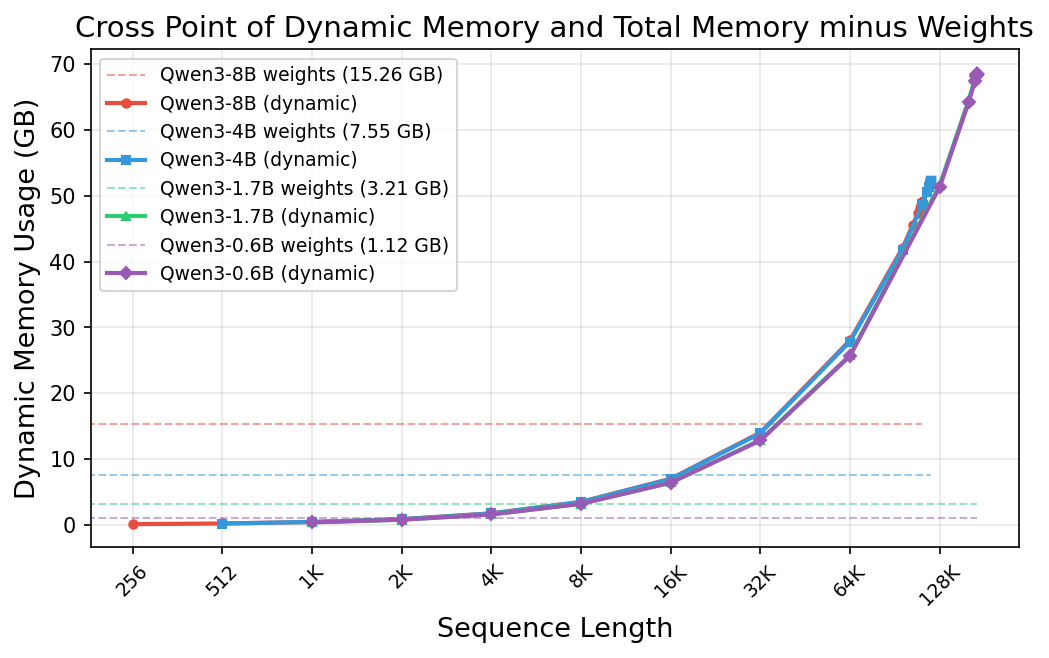
\includegraphics[width=0.5\linewidth]{seq_len_dynamic_memory_crosspoint.png}
    \caption{Dynamic vs. Static memory profile for Qwen3 series}
  \end{figure}
  
\end{frame}


\section{Optimization}

\begin{frame}{Overview}
    \begin{center}
    \small
    \renewcommand{\arraystretch}{1.35}
    \begin{tabular}{lll}
      \toprule
      \textbf{阶段} & \textbf{核心方法} & \textbf{典型技术} \\
      \midrule
      \multirow{5}{*}{Training}
        & \multirow{5}{*}{显存与效率提升}
        & Activation Checkpointing \\
      & & Mixed Precision Training \\
      & & Flash Attention \\
      & & ZeRO \\
      & & Pipeline/Model/Data Parallelism \\
      \midrule
      \multirow{4}{*}{Inference}
        & \multirow{4}{*}{长序列与速度优化}
        & KV Cache Optimization \\
      & & Paged/Radix Attention \\
      & & Faster Attention \\
      & & Quantization \\
      \bottomrule
    \end{tabular}
  \end{center}
\end{frame}



\begin{frame}{Mixed Precision Training}
    \small
  \begin{block}{Motivation}
      计算量大的部分用低精度，计算量小的部分用高精度。低精度参与运算，高精度避免Overflow/Underflow.
  \end{block}
  下图是DeepSeek-V3\cite{deepseekai2025deepseekv3technicalreport}使用的混合精度训练框架
   \begin{figure}
       \centering
       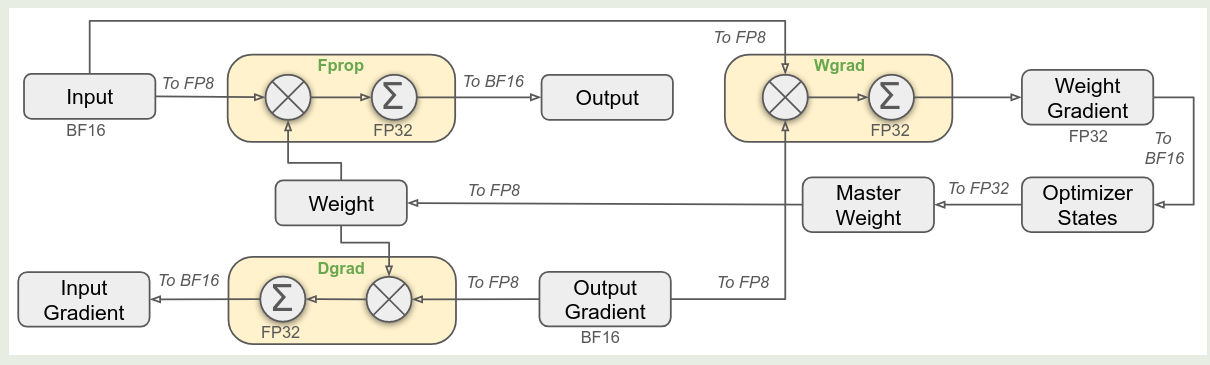
\includegraphics[width=0.7\linewidth]{DeepSeek-V3-mixed-precision.png}
       \caption{Mixed precision training of DeepSeek-V3}
       \label{fig:mid_precision_training}
   \end{figure}
\end{frame}

\begin{frame}{Mixed Precision Training-Analysis}
  \small
  \begin{table}[h]
    \centering
    \begin{tabular}{ccccc}
    \toprule
    \textbf{Precision} & \textbf{BF16} & \textbf{FP32} & \textbf{BF16} \\
    \textbf{AMP} & No & Yes & Yes \\
    \midrule
    Weights & BF16 (2) & FP32 (4) & BF16 (2) \\
    Master weigths & - & - & FP32 (4) \\
    Gradients & BF16 (2) & FP32 (4) & BF16 (2) \\
    Adam m & BF16 (2) & FP32 (4) & FP32 (4) \\
    Adam v & BF16 (2) & FP32 (4) & FP32 (4) \\
    \midrule
    Static total (bytes/param) & 8 & 16 & 16 \\
    \bottomrule
    \end{tabular}
    \caption{Comparison of memory usage per parameter across different training configurations.}
    \label{tab:memory_usage}
    \end{table}
    \begin{block}{Remark}
      \begin{enumerate}
        \item BF16 (w/ AMP) 与 FP32 (w/ AMP) 的静态显存占用相同，但 BF16 (w/ AMP) 的动态显存占用更低。
        \item 主流框架基本都使用了BF16/FP8 (w/ AMP) 的训练方式。
      \end{enumerate}
    \end{block}
\end{frame}

\begin{frame}{Mixed Precision Training-Experiments}
  Experiments on Qwen3-1.7B, batch size = 1, sequence length = 512.
  \begin{figure}
      \centering
      \begin{minipage}{0.32\textwidth}
          \centering
          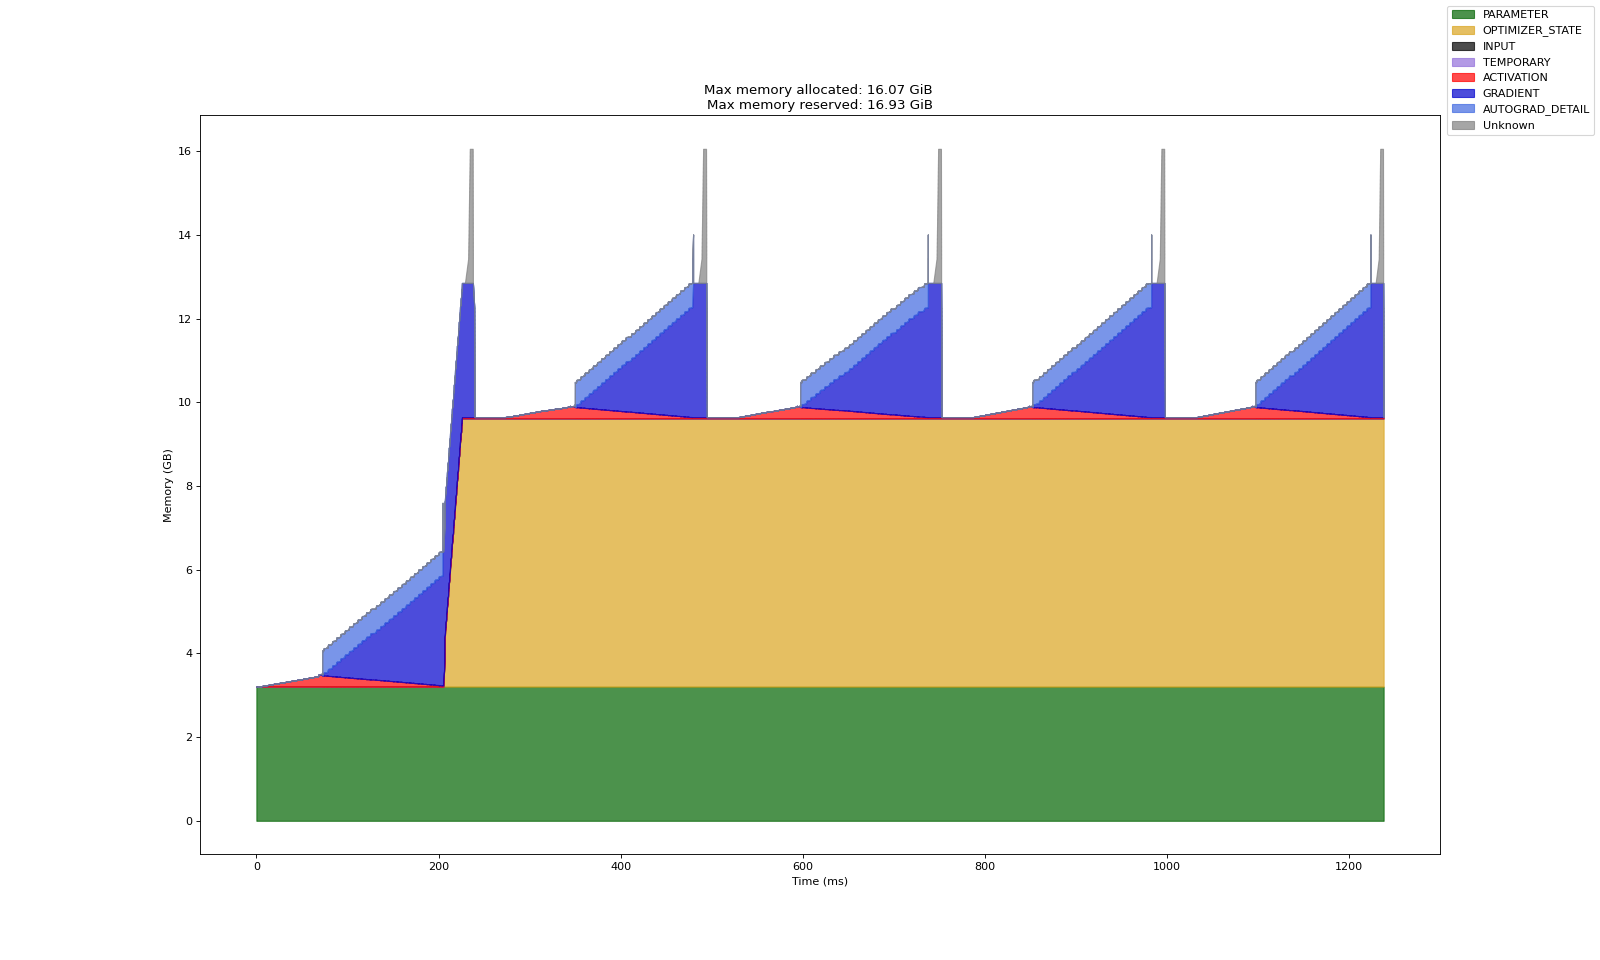
\includegraphics[width=\textwidth]{bf16_wo_amp.png}
          \label{fig:bf16_wo_amp}
      \end{minipage}
      \hfill
      \begin{minipage}{0.32\textwidth}
          \centering
          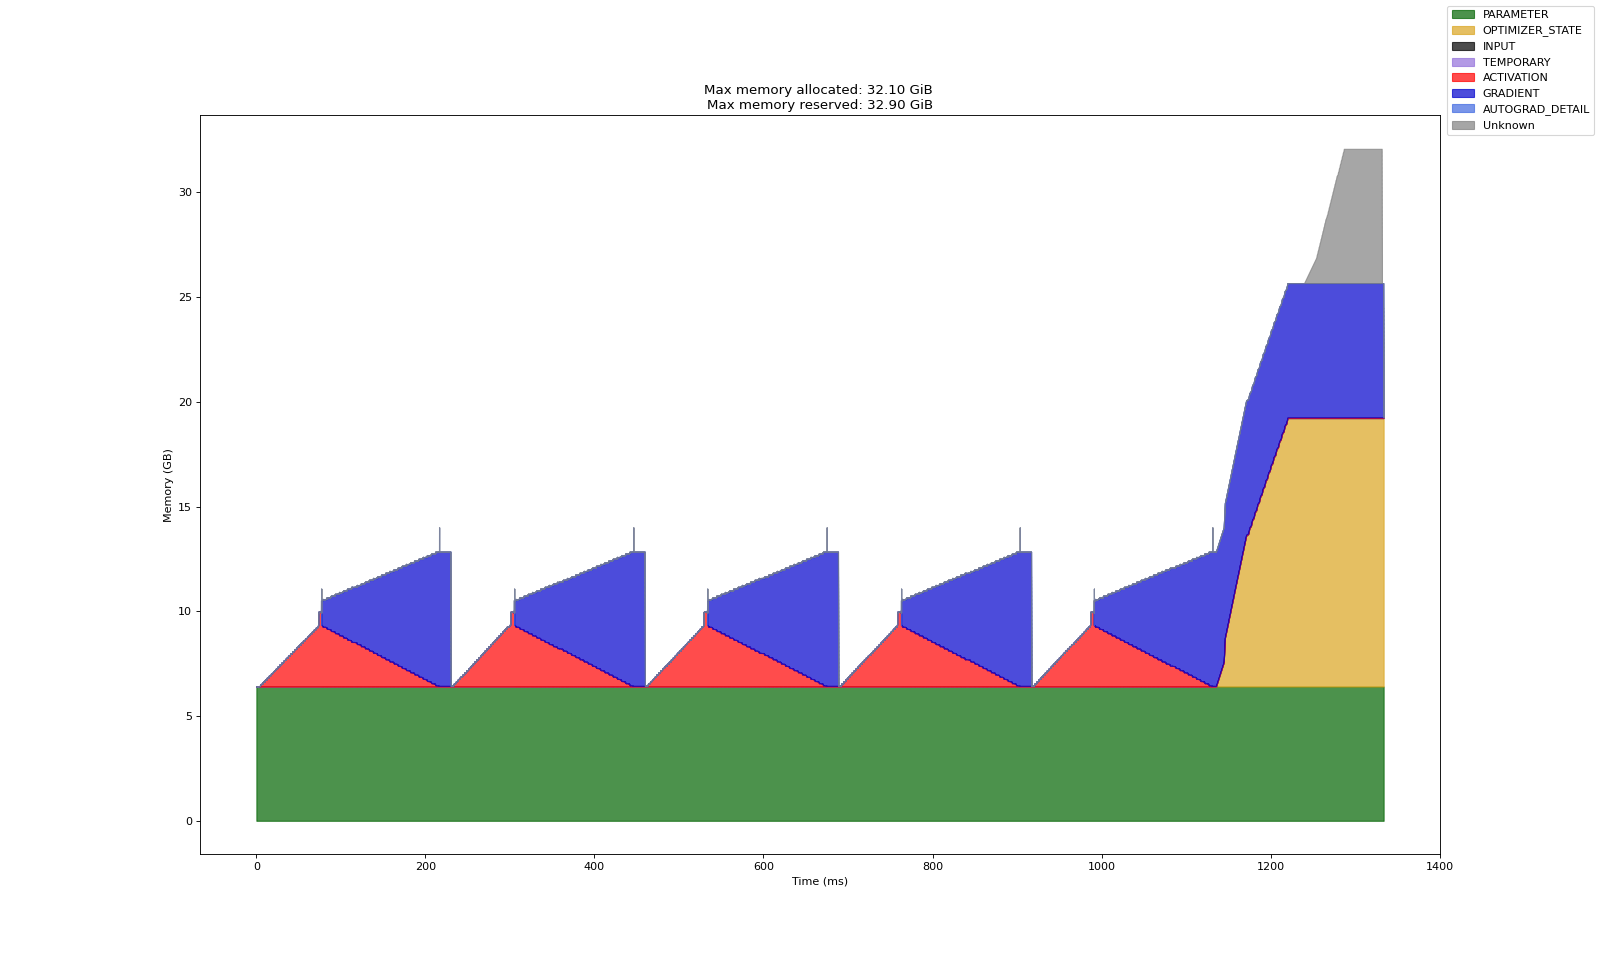
\includegraphics[width=\textwidth]{fp32_w_amp.png}
          \label{fig:fp32_w_amp}
      \end{minipage}
      \hfill
      \begin{minipage}{0.32\textwidth}
          \centering
          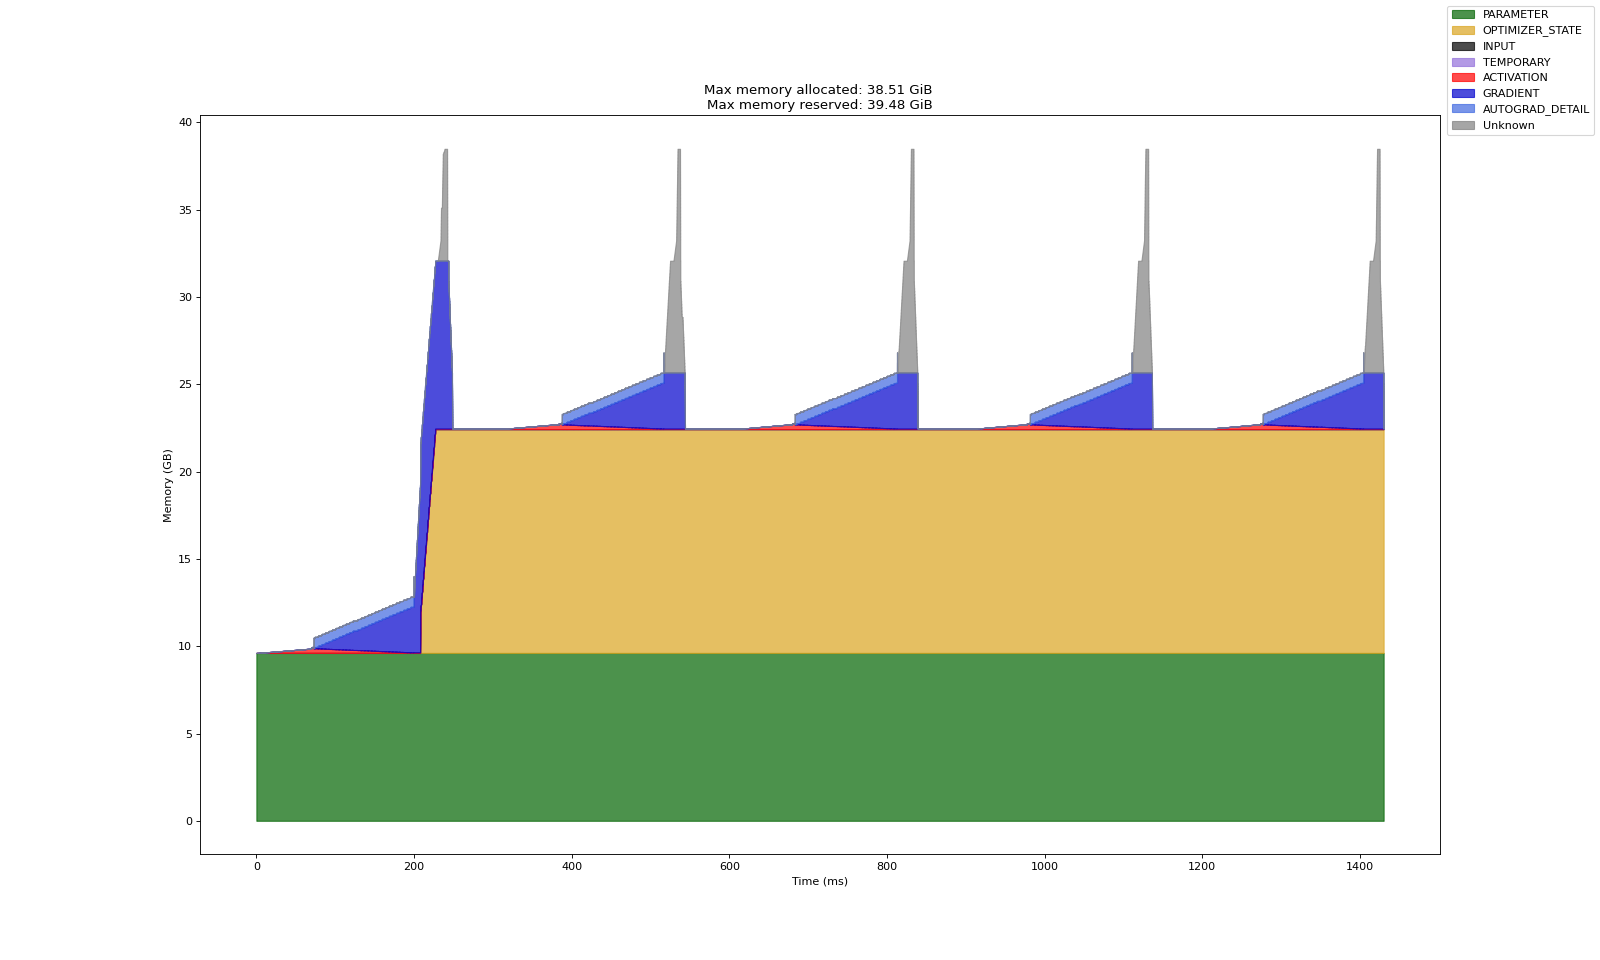
\includegraphics[width=\textwidth]{bf16_w_amp.png}
          \label{fig:bf16_w_amp}
      \end{minipage}
      \caption{(left) BF16 (w/o AMP), $\sim 8P$ bytes, (center) FP32 (w/ AMP), $\sim 16P$ bytes, (right) BF16 (w/ AMP), $\sim 16P$ bytes}
  \end{figure}
\end{frame}


\begin{frame}{ZeRO\cite{rajbhandari2020zeromemoryoptimizationstraining}}
  \small
  \begin{block}{Motivation}
      将 optimizer states / gradients / weights 按不同 GPU 切片存储，需要参与计算时再 all-gather 整合成完整参数。这样每张卡只需维护自己负责的一部分，大幅降低单卡显存需求。
  \end{block}
  
  ZeRO的工作原理如下图所示
  \begin{figure}
      \centering
      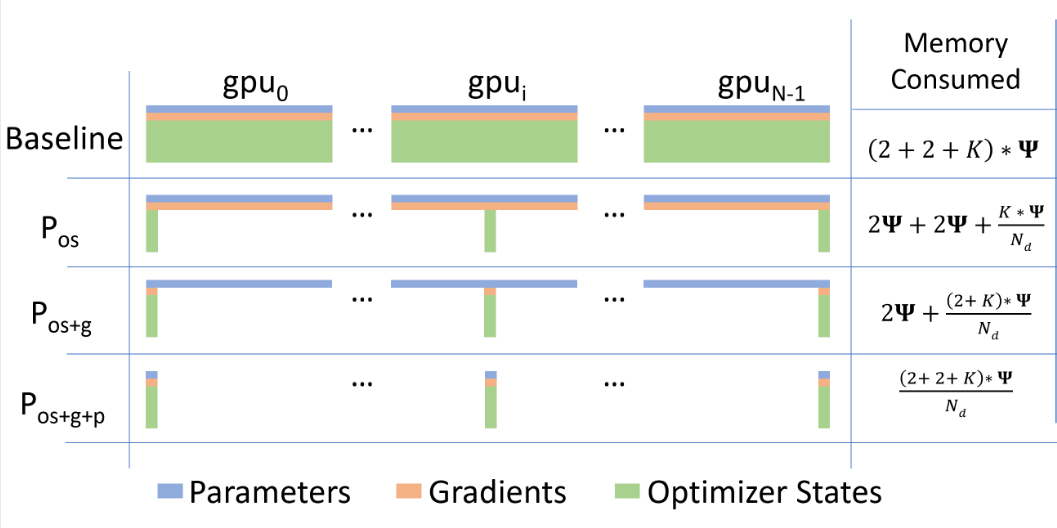
\includegraphics[width=0.5\linewidth]{ZeRO-architecture.png}
      \caption{ZeRO DP framework}
      \label{fig:zero}
  \end{figure}

\end{frame}

\begin{frame}{ZeRO Stages}
    \small
  \begin{itemize}
    \item \textbf{ZeRO1}：shard optimizer states
    \begin{equation}
    \mathrm{Training\_Memory}
    = \mathrm{weight}+\mathrm{activation}
    + \frac{\mathrm{optimizer}}{\#\mathrm{GPUs}}+\mathrm{gradient}
    \tag{ZeRO1}
  \end{equation}
    \item \textbf{ZeRO2}：shard gradients + gradients
  \begin{equation}
    \mathrm{Training\_Memory}
    = \mathrm{weight}+\mathrm{activation}
    + \frac{\mathrm{optimizer}+\mathrm{gradient}}{\#\mathrm{GPUs}}
    \tag{ZeRO2}
  \end{equation}
    \item \textbf{ZeRO3}：shard all
    \begin{equation}
    \mathrm{Training\_Memory}
    = \mathrm{activation}
    + \frac{\mathrm{weight}+\mathrm{optimizer}+\mathrm{gradient}}{\#\mathrm{GPUs}}
    \tag{ZeRO3}
  \end{equation}
  \end{itemize}

    \begin{block}{Remark}
        ZeRO3 可极大降低单卡显存上限，但通信量也会提高。
    \end{block}
\end{frame}

\begin{frame}{Model Parallelism\cite{shoeybi2020megatronlmtrainingmultibillionparameter}}
    \small
    \begin{block}{Motivation}
        将模型切分到不同的GPU上，计算时，先dispatch, 再执行计算，最后通过all-gather等操作得到最终结果。切分方式包括 PP (Pipeline Parallelism), TP (Tensor Parallelism), EP (Expert Parallelism) 等。
    \end{block}
  \begin{equation}
    \mathrm{Training\_Memory}
    = \frac{\mathrm{Memory}(\mathrm{weight})}{\mathrm{PP\ degree} \times \mathrm{TP\ degree}}
  \end{equation}
  
  \vspace{0.2em}
  结合 ZeRO1 与 Model Parallelism 时（activation 中与 TP 相关的部分按 TP degree 缩减）：
  \begin{equation*}
    \mathrm{Memory}_{\mathrm{train}}
    \approx \frac{\mathrm{weight}}{\mathrm{PP}\times\mathrm{TP}}
    + \frac{\mathrm{activation}}{\mathrm{TP}}
    + \frac{\mathrm{optimizer}}{\#\mathrm{GPUs}}
    + \frac{\mathrm{gradient}}{\mathrm{PP}}
  \end{equation*}
\end{frame}


% 补充：可强调「selective 只存每层输入，full 只存模型输入，重算整层/整模型」
\begin{frame}{Activation Checkpointing\cite{korthikanti_reducing_2022}}
  \small
  \begin{block}{Motivation}
    在反向传播时，重新计算所需的输入，来达到以时间换空间的目的。
\end{block}
  \vspace{0.5em}
  \begin{center}
    \small
    \renewcommand{\arraystretch}{1.25}
    \begin{tabular}{lccc}
      \toprule
      & No ckpt & Selective ckpt & Full ckpt \\
      \midrule
      memory & 很高 & 中等 & 很低 $\sim 2bsd$ \\
      extra compute & 无 & 中等 & 很高 $\sim 2Pbs$ \\
      \bottomrule
    \end{tabular}
  \end{center}
  \begin{block}{Remark}
      实践中常结合 model parallelism 与 selective checkpointing 来实现trade off.
  \end{block}
\end{frame}

\begin{frame}{Flash Attention\cite{dao2022flashattentionfastmemoryefficientexact}}
    \small
  \begin{block}{Motivation}
      通过将Attention的计算进行分块，来提高内存访问效率以及降低反向传播时所需要的 activation 大小。
  \end{block}
    
  \textbf{Flash Attention} 通过 tiling 与 online-softmax 降低该部分显存并提升效率\footnote{详见 \href{https://maosong.website/p/notes-on-flashattention/}{notes on Flash Attention}}。这样attention 部分的显存就由 $\mathrm{activation}\propto bs^2$ 降低到了 $\mathrm{activation}\propto bs$. 

  \begin{block}{Theorem}
    flash attention 输出 $O=\mathrm{softmax}(QK^T)V$ (correctness).

    其时间复杂度为 $\mathcal{O}(s^2d)$, 空间复杂度为 $\mathcal{O}(s)$ (memory savings).
  \end{block}
\end{frame}


\begin{frame}{KV Cache Optimization\cite{li2025surveylargelanguagemodel}}
    \begin{equation*}
    \mathrm{Memory}(\mathrm{KV\ cache})
    = s \times 2 \times \redtwo \times L \times h \times d_h
  \end{equation*}
  \begin{enumerate}
      \item $s$: KV cache compression, eviction, selection
      \item $\redtwo$: KV cache quantization
      \item $2$: key-value sharing, MLA\cite{deepseekai2024deepseekv2strongeconomicalefficient}
      \item $h\times d_h$: attention, MQA\cite{shazeer2019fasttransformerdecodingwritehead}, GQA\cite{ainslie2023gqatraininggeneralizedmultiquery}, MLA.
  \end{enumerate}
\end{frame}


\begin{frame}{Weight Quantization}
    \begin{block}{Motivation}
        使用低精度来表示高精度数值的方法，来减少内存占用/提高计算效率。
    \end{block}

    \begin{table}[htbp]
        \centering
        \begin{tabular}{cc}  % 调整为两列
            \toprule
            \textbf{量化时机} & \textbf{代表性工作} \\
            \midrule
            \multirow{4}{*}{训练后量化 (PTQ)} & GPTQ\cite{frantar2023gptqaccurateposttrainingquantization} \\
                                             & AWQ\cite{lin2024awqactivationawareweightquantization} \\
                                             & SmoothQuant\cite{xiao2024smoothquantaccurateefficientposttraining} \\
                                             & GGUF\cite{ggerganov2023ggml} \\
            \midrule
            \multirow{2}{*}{量化感知训练 (QAT)} & LLM-QAT\cite{liu2023llmqatdatafreequantizationaware} \\
                                             & PEQA\cite{kim2023memoryefficientfinetuningcompressedlarge} \\
            \bottomrule
        \end{tabular}
        \caption{大模型量化方法总结}
        \label{tab:quantization_simple}
    \end{table}
\end{frame}

\begin{frame}{Activation Offloading}
    \begin{block}{Motivation}
        将一部分参数/优化器状态/激活值等存储到CPU上，需要的时候再加载到GPU上。
    \end{block}
    \begin{table}[htbp]
        \centering
        \begin{tabular}{cc}
            \toprule
            \textbf{Offloading场景} & \textbf{代表性工作} \\
            \midrule
            \multirow{2}{*}{训练阶段 Offloading} 
                & ZeRO-Offload\cite{ren2021zerooffloaddemocratizingbillionscalemodel} / ZeRO-Infinity \\
                & FSDP\cite{zhao2023pytorchfsdpexperiencesscaling} CPU Offload \\
            \midrule
            \multirow{2}{*}{推理阶段 Offloading} 
                & FlexGen\cite{sheng2023flexgenhighthroughputgenerativeinference} \\
                & vLLM\cite{kwon2023efficient} KV Cache Offload \\
            \midrule
            \multirow{2}{*}{MoE Offloading} 
                & KTransformers\cite{KTransformers} \\
                & DeepSpeed-MoE\cite{rajbhandari2022deepspeedmoeadvancingmixtureofexpertsinference} \\
            \bottomrule
        \end{tabular}
        \caption{offloading methods}
        \label{tab:offloading_methods}
    \end{table}
\end{frame}



\section{Real Systems}

\begin{frame}{Training}
    \begin{table}[]
    \centering
    \begin{tabular}{ccc}
    \toprule
    \textbf{Framework} &  \textbf{Memory Optimizations}                                      \\ \midrule
    Megatron-LM\cite{shoeybi2020megatronlmtrainingmultibillionparameter}                  & TP, SP, Activation Checkpointing \\ \midrule
    DeepSpeed\cite{deepspeed2020systemoptimizationsenabletrainingdeeplearningmodelswithover100billionparameters}                     & ZeRO-1/2/3, CPU/NVMe Offload, Activation Checkpointing             \\ \midrule
    FSDP\cite{zhao2023pytorchfsdpexperiencesscaling}         & Full parameter sharding, Gradient sharding, CPU Offload            \\ \midrule
    Colossal-AI\cite{colossalai2023aunifieddeeplearningsystemforlargescaleparalleltraining}            & ZeRO, TP, PP, Activation Checkpointing                             \\ \midrule
    \end{tabular}
    \end{table}
\end{frame}


\begin{frame}{Inference}
    \begin{table}[]
    \centering
    \begin{tabular}{lll}
    \toprule
    \textbf{Framework} & \textbf{Key Techniques} & \textbf{Memory Optimizations}              \\ \midrule
    vLLM\cite{kwon2023efficient}               & Paged Attention         & KV cache paging, Continuous batching       \\ \midrule
    SGLang\cite{sglang2024efficientexecutionofstructuredlanguagemodelprograms}             & Radix Attention         & KV cache reuse, Efficient scheduling       \\ \midrule
    TensorRT-LLM\cite{tensorrt-llm2023}       & Kernel fusion           & Weight quantization, KV cache optimization \\ \midrule
    \end{tabular}
    \end{table}
\end{frame}


\section{Conclusion}

\begin{frame}{Takeaway}
    \begin{center}
    \small
    \renewcommand{\arraystretch}{1.3}
    \begin{tabular}{cccc}
      \toprule
      \textbf{Components} & \textbf{Training}  & \textbf{Inference} & \textbf{Optimization}             \\\midrule
      weights             & $2P$               & $2P$               & quantization                      \\\midrule
      optimizer states    & $4P$              & 0                  & ZeRO, offloading                  \\\midrule
      gradients           & $2P$               & 0                  & ZeRO                              \\\midrule
      activations         & $\sim 4Lhs^2b$     & $\sim 0.4P$        & ckpt, offloading, flash attention \\\midrule
      KV cache            & 0                  & $4sLhd_h$          & kv optimization, attention        \\\midrule
      TOTAL               & $8P+4Lhs^2b$ & $2.4P+4sLhd_h$     &                                   \\ 
      \bottomrule
    \end{tabular}
  \end{center}
  \begin{itemize}
    \item \textbf{训练}：瓶颈主要在激活值（随 batch size / 序列长度线性增长）。
    \item \textbf{推理}：瓶颈主要在 KV Cache（随序列长度增长）。
  \end{itemize}
\end{frame}



\begin{frame}{Conclusion \& Future Directions}
    \begin{block}{Conclusion}
        We discussed how to analyze the memory occupied by an LLM and how to optimize it.
    \end{block}

    \begin{block}{Future Directions}
        \begin{enumerate}
            \item More efficient architecture (attention, MoE).
            \item Scalable training/inference framework
            \item Software-hardware co-design algorithms.
        \end{enumerate}
    \end{block}
\end{frame}




% ===========================================================================
\section{References}
% ===========================================================================


\begin{frame}[allowframebreaks]
    \frametitle{References}
    \bibliographystyle{amsalpha}
    \bibliography{reference.bib}
\end{frame}

% \begin{frame}{References}
%   \footnotesize
%   \begin{itemize}
%     \item \href{https://blog.eleuther.ai/transformer-math/}{transformer-math} (EleutherAI)
%     \item \href{https://kipp.ly/transformer-inference-arithmetic/}{transformer inference arithmetic}
%     \item Reducing Activation Recomputation in Large Transformer Models (arXiv:2205.05198)
%     \item A Survey on Large Language Model Acceleration based on KV Cache Management (arXiv:2412.19442)
%     \item Efficient Large Language Models: A Survey (arXiv:2312.03863)
%     \item \href{https://maosong.website/p/notes-on-adamw/}{notes on AdamW}, \href{https://maosong.website/p/notes-on-flashattention/}{notes on Flash Attention}
%   \end{itemize}
% \end{frame}

\end{document}
